\begin{frame}{Projekt - Idee}
  \begin{center}
    
\includegraphics[width=0.9\textwidth]{images/grobarchitektur}
  \end{center}
\end{frame}

\section{Was wir dann gemacht haben}

\begin{frame}{Projekt - Realität}
  \begin{center}
    
\includegraphics[width=0.9\textwidth]{images/realworld}
  \end{center}
\end{frame}

\begin{frame}{deCONZ - REST-API - GET 1/2}
  \Large
  GET-Requests: Informationsbeschaffung
  \center{
    \begin{tabular}{ l l }
      \texttt{<url>/<apikey>} & \\
      Lichter & \texttt /\alert{\texttt{lights}}\\
      Gruppen & \texttt /\alert{\texttt{groups}}\\
      Szenen & \hspace{1em}$\looparrowdownright$\hspace{1em}
        \texttt{/<id>/\alert{\texttt{scenes}}}\\
    \end{tabular}
  }
  \flushleft
  für \alert{alle} Lichter, Gruppen und Szenen.
\end{frame}

\begin{frame}{deCONZ - REST-API - GET 2/2}
  \Large
  GET-Requests: Informationsbeschaffung
  \center{
    \begin{tabular}{ l l }
      \texttt{<url>/<apikey>} & \\
      Lichter & \texttt /\alert{\texttt{lights/<id>}}\\
      Gruppen & \texttt /\alert{\texttt{groups/<id>}}\\
      Szenen & \hspace{1em}$\looparrowdownright$\hspace{1em}
        \texttt /\alert{\texttt{scenes/<id>}}\\
    \end{tabular}
  }
  \flushleft
  für \alert{einzelne} Lichter, Gruppen und Szenen
\end{frame}

\begin{frame}{deCONZ - REST-API - PUT}
  \Large
  PUT-Requests: Datenaktualisierung
  \center{
    \begin{tabular}{ l l }
      \texttt{<url>/<apikey>} & \\
      Lichter & \texttt /\alert{\texttt{lights/<id>/state}}\\
      Gruppen & \texttt /\alert{\texttt{groups/<id>}}\\
      Szenen & \hspace{1em}$\looparrowdownright$\hspace{1em}
        \texttt /\alert{\texttt{scenes/<id>}}\\
    \end{tabular}
  }
  \flushleft
  für \alert{einzelne} Lichter, Gruppen und Szenen
\end{frame}

\begin{frame}{deCONZ - REST-API - POST}
  \Large
  POST-Requests: Erstellung
  \center{
    \begin{tabular}{ l l }
      \texttt{<url>/<apikey>} & \\
      Gruppen & \texttt /\alert{\texttt{groups}}\\
      Szenen & \hspace{1em}$\looparrowdownright$\hspace{1em}
        \texttt{/<id>/\alert{\texttt{scenes}}}\\
    \end{tabular}
  }
  \flushleft
  von Gruppen und Szenen
\end{frame}

\begin{frame}{deCONZ - REST-API - DELETE}
  \Large
  DELETE-Requests: Löschung
  \center{
    \begin{tabular}{ l l }
      \texttt{<url>/<apikey>} & \\
      Gruppen & \texttt /\alert{\texttt{groups}}\\
      Szenen & \hspace{1em}$\looparrowdownright$\hspace{1em}
        \texttt{/<id>/\alert{\texttt{scenes}}}\\
    \end{tabular}
  }
  \flushleft
  von Gruppen und Szenen
\end{frame}

\begin{frame}{}
  \begin{center}
    \vspace{-0.2cm}
    \makebox[\textwidth][c]{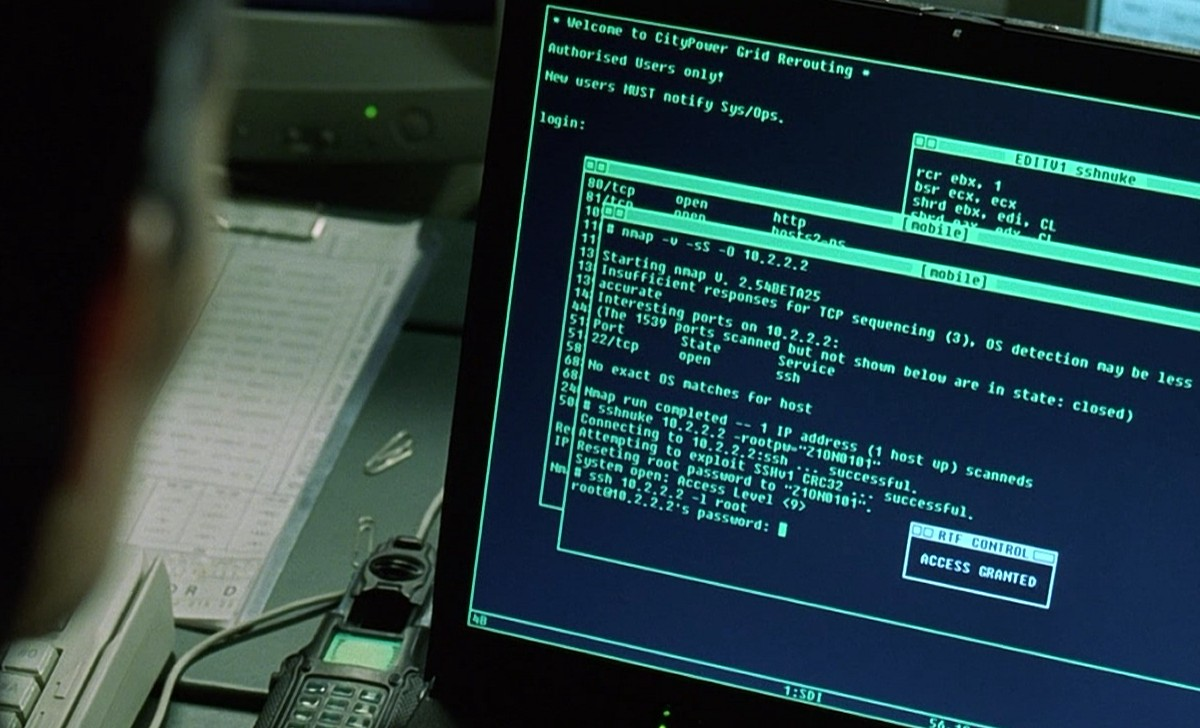
\includegraphics[width=1.25\paperwidth]{images/matrix}}
    \label{fig:matrix}
  \end{center}
\end{frame}

\begin{frame}{CLI - lolo}
  \Large
  \begin{itemize}
    \item Command-Line-Interface
    \item Ruby
    \item clamp
    \item rest-client
    \item nutzt deCONZ Rest-API
  \end{itemize}
\end{frame}